%!TEX program = Xelatex
\documentclass{article}
%\usepackage{ctex}
\usepackage{amsmath,amscd,amsbsy,amssymb,latexsym,url,bm,amsthm}
\usepackage{epsfig,graphicx,subfigure}
\usepackage{enumitem,balance,mathtools}
\usepackage{wrapfig}
\usepackage{mathrsfs, euscript}
\usepackage[usenames]{xcolor}
\usepackage{hyperref}
\usepackage{caption}
%\usepackage{subcaption}
\usepackage{float}
\usepackage{listings}
%\usepackage{enumerate}
%\usepackage{algorithm}
%\usepackage{algorithmic}
%\usepackage[vlined,ruled,commentsnumbered,linesnumbered]{algorithm2e}
\usepackage[ruled,lined,boxed,linesnumbered]{algorithm2e}

\newtheorem{theorem}{Theorem}[section]
\newtheorem{lemma}[theorem]{Lemma}
\newtheorem{proposition}[theorem]{Proposition}
\newtheorem{corollary}[theorem]{Corollary}
\newtheorem{exercise}{Exercise}[section]
\newtheorem*{solution}{Solution}

\renewcommand{\thefootnote}{\fnsymbol{footnote}}

\newcommand{\postscript}[2]
    {\setlength{\epsfxsize}{#2\hsize}
    \centerline{\epsfbox{#1}}}

\renewcommand{\baselinestretch}{1.0}

\setlength{\oddsidemargin}{-0.365in}
\setlength{\evensidemargin}{-0.365in}
\setlength{\topmargin}{-0.3in}
\setlength{\headheight}{0in}
\setlength{\headsep}{0in}
\setlength{\textheight}{10.1in}
\setlength{\textwidth}{7in}

\title{CS222 Homework 2}
\author{Algorithm Analysis \& Deadline: 2020-9-28 Monday 24:00}
\date{Exercises for Algorithm Design and Analysis by Li Jiang, 2020 Autumn Semester}

\begin{document}

\maketitle

\begin{enumerate}

\item Consider the following job scheduling problem. We are given all at once N jobs with positive lengths $l_1$,$l_2$,…,$l_n$. We can schedule only one job at a time and once we start a job we must run it to completion. A schedule for a set of jobs is then the starting time for each job $s_1$,$s_2$,…,$s_n$. Find an efficient algorithm to schedule the jobs to minimize the total wait time, where the wait time for a job is the difference between the time the job arrived and when it finished. Since all jobs arrive at the same time $t=0$, the wait time for job $i$ simplifies to $l_i+s_i$ and so the problem is to schedule the jobs to minimize $\sum _{i=1}^{i=n} (l_i + s_i)$. Please design an algorithm based on greedy strategy to solve the above problem(Write a pseudocode) and prove that your algorithm is correct.\\

~\\
\begin{solution}
    We need to minimize $\sum_{i=1}^n s_i$ because $l_i$ are fixed values. And a natural strategy is to schedule jobs with short lengths first.\\
    \begin{minipage}[t]{0.8\textwidth}
        \begin{algorithm}[H]
            \KwIn{$l_1,l_2,\cdots,l_n$}
            \KwOut{$s_1,s_2,\cdots,s_n$}
    
            \BlankLine
            \caption{Greedy-short-length-first}\label{Alg-greedy1}
            Sort $n$ jobs so that $l_1\leq l_2\leq \cdots \leq l_n$\\
            $t \leftarrow 0$\\
            \For{$j \leftarrow 1$ \KwTo $n$}{
                Schedule job $j$ to start at $s_j = t$\\
                $s_j \leftarrow t$\\
                $t \leftarrow t + l_j$\\
            }
            \Return{$s_1,s_2,\cdots,s_n$}          
        \end{algorithm}
        \end{minipage}\\
    \begin{enumerate}
        \item Correct: $s_{j+1}-s_{j} = l_j$ according to the algorithm. So no two jobs run at the same time.
        \item Optimal: Obviously the optimal solution must have no idle time. Assume there is an optimal solution $S^*$ different to the solution got from our greedy algorithm above. There must be such adjacent $i, j$ that $s_i < s_j, l_i > l_j$ in $S^*$.
            We exchange job $i$ with job $j$. Then the total wait time decreases by $\delta_t=l_i-l_j>0$. So solution $S^*$ cannot be optimal. Contradict! So the optimal solution must have a ascending order of $l_i$, hence our greedy algorithm above will get the optimal solution.
            \begin{figure}[!h]
                \centering
                \caption{sketch map for problem 1}
                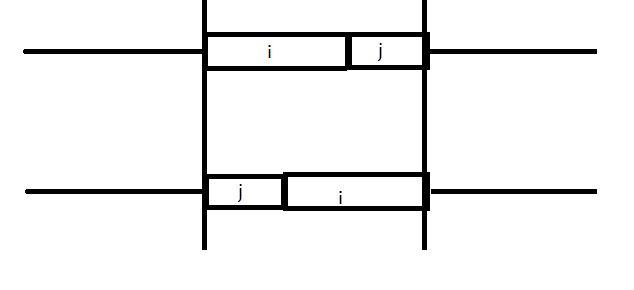
\includegraphics[width=0.5\textwidth]{example1.png}
            \end{figure}
        \item Efficient: $T(n)=\Theta(n\log n)$.
    \end{enumerate}
\end{solution}
~\\


Consider the above problem, but associate with the jobs positive values of importance $w_1,…,w_n$, and minimize $\sum_{i=1}^{i=n} w_i(l_i+s_i)$. Find an efficient algorithm to determine an optimal schedule in this case. Please design an algorithm based on greedy strategy to solve the above problem(Write a pseudocode). You need not prove that your algorithm is correct.

~\\
\begin{solution} Sort by $\dfrac{l_i}{w_i}$.\\
    \begin{minipage}[t]{0.8\textwidth}
        \begin{algorithm}[H]
            \KwIn{$l_1,l_2,\cdots,l_n$}
            \KwOut{$s_1,s_2,\cdots,s_n$}
    
            \BlankLine
            \caption{Greedy-smallest-l/w-first}\label{Alg-greedy2}
            Sort $n$ jobs so that $\dfrac{l_1}{w_1}\leq \dfrac{l_2}{w_2}\leq \cdots \leq \dfrac{l_n}{w_n}$\\
            $t \leftarrow 0$\\
            \For{$j \leftarrow 1$ \KwTo $n$}{
                Schedule job $j$ to start at $s_j = t$\\
                $s_j \leftarrow t$\\
                $t \leftarrow t + l_j$\\
            }
            \Return{$s_1,s_2,\cdots,s_n$}          
        \end{algorithm}
        \end{minipage}\\
\end{solution}
~\\

\item Considering the following Problem, and show your algorithm with pseudocode. Please ensure that the complexity of your algorithm is $O(n)$.\\
You have an array “prices” for which the $ith$ element is the price of a given stock on day $i$. Design an algorithm to find the maximum profit. You may complete as many transactions as you like (i.e., buy one and sell one share of the stock multiple times).\\

Note: You may not engage in multiple transactions at the same time (i.e., you must sell the stock before you buy again).

Example1: the input array is : [7,1,5,3,6,4]. The output of the maximum profit is 7.\\


~\\
\begin{solution} Assume $p_i$ is monotone increasing in intervals $[l_1,r_1],[l_2,r_2],\cdots,[l_k,r_k]$. The optimal solution is $profit = \sum_{i=1}^k p_{r_i}-p_{l_i}=\sum_{i=2}^n \max\{0, p_i-p_{i-1}\}$, because it can be checked easily that buying at $l_i$ and selling at $r_i$ is better than buying at $l_i+\epsilon_{l_i}$ and selling at $r_i+\epsilon_{r_i}$.\\
    \begin{minipage}[t]{0.8\textwidth}
        \begin{algorithm}[H]
            \KwIn{$p_1,p_2,\cdots,p_n$}
            \KwOut{$profit$}
    
            \BlankLine
            \caption{Greedy-low-buy-high-sell}\label{Alg-greedy3}
            $profit \leftarrow 0$\\
            \For{$i \leftarrow 2$ \KwTo $n$}{
                $profit \leftarrow profit + \max\{0, p_i-p_{i-1}\}$
            }
            \Return{$profit$} 
        \end{algorithm}
    \end{minipage}\\
    $T(n)=O(n)$
\end{solution}
~\\

\item Consider the following Interval Problem. \\
INPUT:A set $S = \{(x_i, y_i)|1 \leq  i \leq  n\}$ of intervals over the real line. Think of interval $(x_i
, y_i)$ as being a request for a room for a class that meets from time $x_i$ to time $y_i$.\\
OUTPUT: Find an assignment of classes to rooms that uses the fewest number of rooms.\\
\textbf{Note:} that every room request must be honored and that no two classes can use a room at the same
time.\\

Consider the following iterative algorithm. Assign as many classes as possible to the first room(sorted by end time), then assign as many classes as possible to the second room, then assign as many classes as possible to the third room, etc. Is this algorithm correct? Prove the correctness of such idea, or else provide a counter-example, and design your algorithm.\\
   

~\\
\begin{solution}
    This algorithm described above (sort by end time in ascending order) is not optimal. Counterexample:\\
    Consider intervals $(1,3),(2,5),(6,7),(4,8)$. The solution got by the algorithm above is classroom1: $(1,3),(6,7)$, classroom2: $(2,5)$, classroom3: $(4,8)$. Need 3 rooms.
    However, a better solution is classroom1: $(1,3),(4,8)$, classroom2: $(2,5),(6,7)$. Need 2 rooms.\\
    \begin{figure}[!h]
        \centering
        \caption{Counterexample for problem 3}
        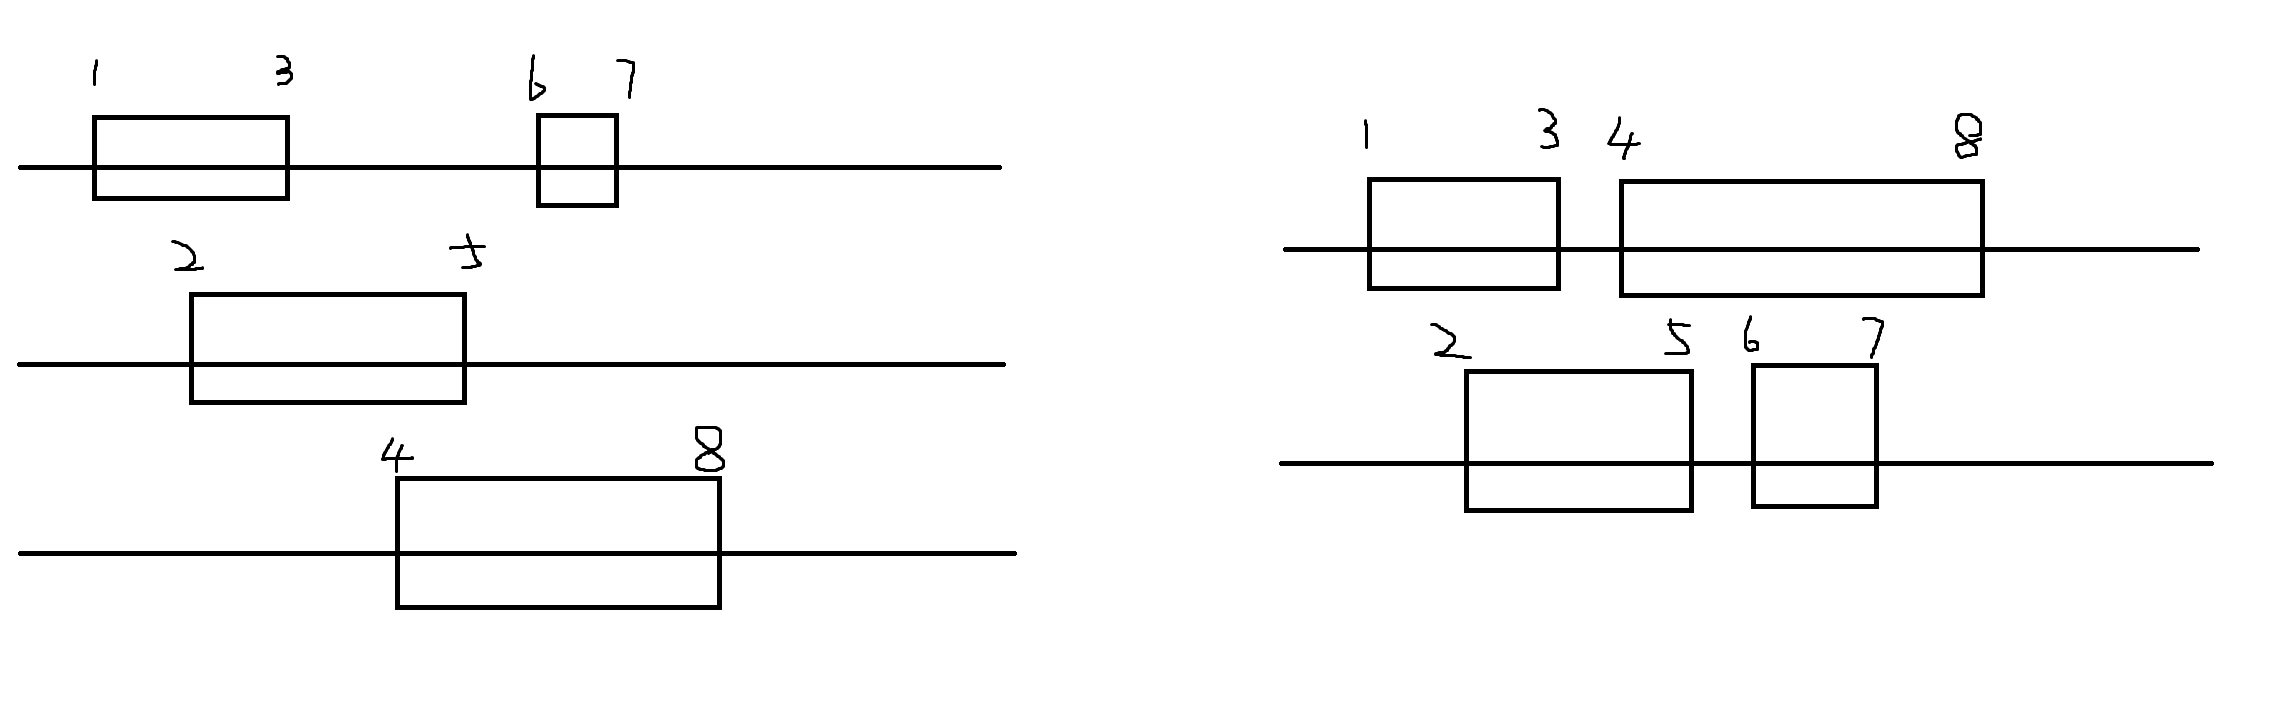
\includegraphics[width=0.8\textwidth]{example2.png}
    \end{figure}\\
    My algorithm: sort the classes by start time. If a class can be add to a classroom, then add it. If a class conflicts with all the classroom allocated, then allocate a new classroom and add this class into it.\\
    \begin{minipage}[t]{0.8\textwidth}
        \begin{algorithm}[H]
            \caption{Greedy-start-time-early-first}\label{Alg-greedy4}
            \KwIn{$(x_1,y_1),(x_2,y_2),\cdots,(x_n,y_n)$}
            \KwOut{$class_1,class_2,\cdots,class_n$}
    
            \BlankLine
            
            $number \leftarrow 0$\\
            \For{$i\leftarrow 1$ \KwTo $n$}{
                $assigned\leftarrow $ false.\\
                Try to assign a room.\\
                \For{$j\leftarrow 1$ \KwTo $number$}{
                    \If{$end_j\leq x_i$}{
                        $class_i \leftarrow j$\\
                        $end_j \leftarrow y_i$\\
                        $assigned \leftarrow $ true\\
                        \rm{\textbf{break}}
                    }
                }
                \If{$assigned$ = false}{
                    Allocate a new room.\\
                    $number$ = $number$ + 1\\
                    $class_i\leftarrow number$\\
                    $end_{number}\leftarrow y_i$\\
                }
            }
            \Return{$class_1,class_2,\cdots,class_n$} 
        \end{algorithm}
    \end{minipage}\\
    The correctness and the optimality are proved in the class. The main proving strategy is to show there are $\$number$ lessons cover each other in certain interval, hence the number of rooms needed cannot be less than $\$number$. $T(n)=\Theta(n^2)$, using binary heap can reduce it to $\Theta(n\log n)$.
    \vspace{10pt}
    \\
    However, if sort by end time in descending order, and assign as many classes as possible, then it is optimal. The proving strategy is similar to the one above. Assume that we use $d$ classrooms. And there is a class $t : (x_t,y_t)$ in classroom $d$. Class $t$ is incompatible with a class $t_i$ in classroom $i,\ 1\leq i < d$. We claim that $\forall 1\leq i < d, x_{t_i} < y_t$ and $y_{t_i} \geq y_t$, because class $t$ is incompatible with class $t_i$ and $t$ is assigned after $t_i$. So there is at least $d$ classes cover each other in the non-empty interval $(\max\{\max\{x_{t_i}\}, x_t\}, y_t)$. So $d$ is the least number of classrooms needed, the algorithm is optimal.
\end{solution}
~\\


\item Considering the following Problem, and show your algorithm with pseudocode. Please ensure that the complexity of your algorithm is $O(n)$.\\
Given an array of non-negative integers, you are initially positioned at the first index of the array. Each element in the array represents your maximum jump length at that position. Your goal is to reach the last index in the minimum number of jumps.\\

Note:You can assume that you can always reach the last index.

\textbf{Example1:} Input: [2,3,1,1,4]; Output: 2
Explanation: The minimum number of jumps to reach the last index is 2. Jump 1 step from index 0 to 1 (in index 0 you can choose to jump to index1 or index2), then 3 steps to the last index(in index 1 you can jump to index2, index3 or index4).

~\\

\begin{solution}
    Assume now we are at position $i$, and we can jump to the position $i+1, \cdots, i+a_i$. Which target position is the best? If $i+1\leq s, t\leq i+a_i$ and $s+a_s < t+a_t$, then the target $t$ is better than $s$, because any position can be reached from $s$ by 1 step can be also reached from $t$ by 1 step. So our strategy is to choose the target $i<j\leq i+a_i$ with the largest jump range $j+a_j$.\\
    \begin{minipage}[htb]{0.8\textwidth}
        \begin{algorithm}[H]
            \caption{greedy-largest-jump-range-first}
            \label{Alg-jump}
            \KwIn{$a_1,a_2,\cdots,a_n$}
            \KwOut{$minjump$}
            \BlankLine
            $goal \leftarrow n$\\
            $pos \leftarrow 1$\\
            $i \leftarrow pos + 1$\\
            $tojump \leftarrow i$\\
            $minjump \leftarrow 0$\\
            \While{$pos < goal$}{
                \If{$i=goal$}{
                    $pos\leftarrow i$\\
                    $minjump\leftarrow minjump + 1$\\
                    \rm{\textbf{break}}
                }
                \If{$i+a_i > tojump + a_{tojump}$}{
                    $tojump \leftarrow i$
                }
                \If{$i = pos+a_{pos}$}{
                    $pos\leftarrow tojump$\\
                    $minjump\leftarrow minjump + 1$
                }
                $i\leftarrow i + 1$
            }
            \Return{$minjump$}
        \end{algorithm}
    \end{minipage}\\
    Some property: 
    \begin{enumerate}
        \item If jump from $i$ to $j$, then $i+a_i < j+a_j$. Reason: First we say $i+a_i \leq (i+a_i)+a_{i+a_i}\leq j+a_j$; Second if $i+a_i = j+a_j$ we cannot jump to the goal in any jumping strategy.
        \item To find the best target $t$ to jump from $j$, we only consider the positions after $i+a_i$, because all the positions $t'$ before $i+a_i$ satisfy $t'+a_{t'} \leq j+a_j \leq (j+a_j)+a_{j+a_j}\leq t+a_t$.
        \item $T(n)=\Theta(n)$. In every iteration, variable $i$ increases by $1$. When $i$ reaches $goal=n$, the loop finishes. Hence it iterates at most $n$ times.
    \end{enumerate}
    
\end{solution}


\end{enumerate}

\end{document}
